\documentclass[10pt]{article}
% Workshop 2 report, DRAFT.  Section letters follow Deliverable 2; adapt to the Workshop 2
% template once it is announced.  Numbers marked (interim) come from laptop runs still in
% progress on Nov 16 and are to be replaced by slurm/workshop2.sh.
\usepackage[margin=0.7in]{geometry}
\usepackage{amsmath,amssymb}
\usepackage{booktabs}
\usepackage{enumitem}
\usepackage{graphicx}
\usepackage[T1]{fontenc}
\usepackage[hidelinks]{hyperref}
\usepackage{caption}
\captionsetup{font=small,labelfont=bf,skip=2pt}
\setlist{nosep,leftmargin=1.2em}
\graphicspath{{../results/}{../results/live_2026_10/}}
\setlength{\parskip}{2pt}
\newcommand{\Fanon}{\mathcal{F}^{\mathrm{anon}}}
\newcommand{\Fid}{\mathcal{F}^{\mathrm{id}}}
\newcommand{\LBR}{L_{\mathrm{BR}}}
\newcommand{\sect}[1]{\par\vspace{6pt}\noindent\textbf{#1}\par\vspace{1.5pt}\noindent}

\title{\vspace{-1.6em}{\Large\textbf{Rent or Toxicity? Strategic Exploitability of Learning Market Makers\\ with Public Wallet Information}}\\[0.15em]\large Wargame Deliverable 3: Workshop 2 report (draft)}
\author{Deepu Pradeep \quad Miguel Betran Menz\\
\normalsize 6.S974 Games, Learning, and Security. Example 4: Algorithmic Market with Adaptive Agents}
\date{November 2026}

\begin{document}
\maketitle
\vspace{-2em}

\sect{a) Where we stood, and what Workshop 2 was for}
\textbf{The setting in four sentences.} \emph{Market makers} post standing offers to buy and sell around a reference price (the \emph{mid}); the gap between their prices is the \emph{spread}, measured here as a \emph{half-spread} $h$ in \emph{ticks} (the smallest price step). \emph{Takers} accept those offers; some are \emph{informed} (they trade only when the maker loses), and the informed share of a flow is its \emph{toxicity}. Learning makers settle on a spread wider than the \emph{break-even} (Nash) quote $h^C$ without communicating; such a set is a \emph{cartel}, what it earns above the Nash profit is its \emph{rent}, and the \emph{rent index} $C$ places it between Nash (0) and joint monopoly (1). An \emph{entrant} is an adversarial maker added to a trained cartel; \emph{rent units} divide any profit by the gap between monopoly and Nash profit.

\textbf{Workshop 1} showed that the rent exists ($C=0.78$--$0.86$), that the \emph{exact best response} of an entrant who knows the cartel's \emph{reaction function} (its map from last period's quotes to its next quotes) takes all of it, that public wallet identity has value through spells of informed trading rather than through wallet persistence, and that on Hyperliquid the makers who earn are the ones who avoid previously toxic wallets. The feedback on that report asked for no changes and endorsed the plan, which had four items: (1) an attacker with public information only; (2) both sides learning; (3) attacks when the spread is pinned at one tick (the \emph{queue game}); (4) all defences on one frontier. This report answers them in that order. The new terms are: \emph{probing budget} (periods the attacker spends quoting at random to observe reactions), \emph{double oracle} (each side in turn best-responds to the other), \emph{request allowance} (the venue's cap on how many orders an address may place, earned back by trading), and \emph{fringe} (makers that always keep an order standing and cannot see who they trade with).

\sect{b) Results}
\textbf{b1. The attack needs only public information} (60 cartels, two and three makers; final). Every value of the reaction function is visible on the public book, and the entrant can set the rival quote the cartel reacts to. An entrant that records the function cell by cell and solves its estimate earns $1.06$--$1.15$ rent units after 200 probing periods and matches the exact best response ($1.08$--$1.21$) to the second decimal after 1000, for two and for three incumbents. Probing costs profit, so the best budget is two to ten episodes.

\textbf{b2. A cartel that keeps learning destroys its rent and does not defend it} (15 two-maker cartels; Figure~\ref{fig:relearn}). The cartel resumes learning under attack for 3000 episodes. While it learns, an oracle that re-solves from the cartel's current tables earns $0.45$--$0.64$ rent units instead of $1.1$, because the exploring cartel quotes tighter; the public attacker stays within $0.05$ of the oracle throughout and returns to $1.12$ (oracle $1.13$) once the cartel stops. The cartel's own profit is at or slightly below the Nash level the whole time ($-0.09$ to $-0.01$). Forgetting old observations, the design we proposed for a drifting target, makes the attacker \emph{worse} by $0.01$--$0.06$. Only a stale attacker that never re-solves leaves the cartel anything ($0.05$--$0.13$).

\begin{figure}[h]\centering
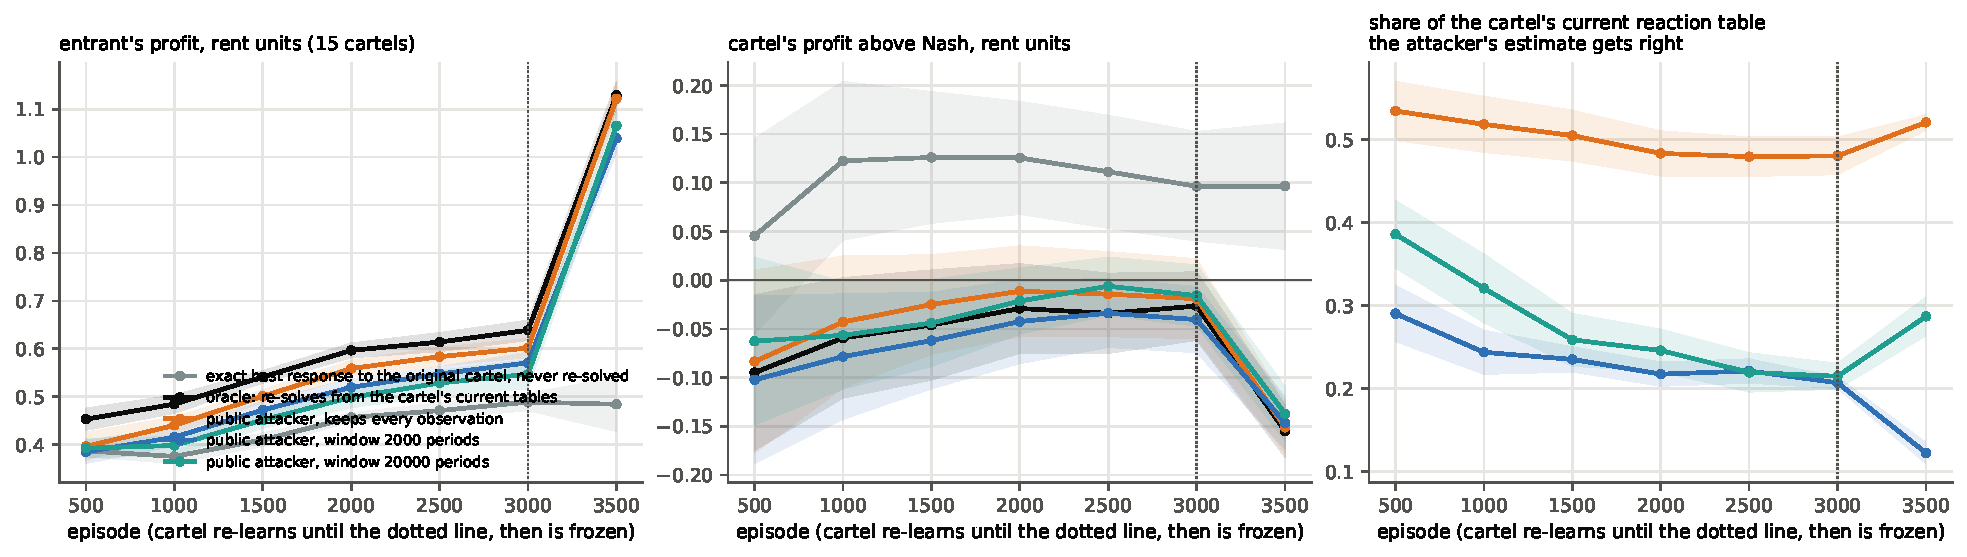
\includegraphics[width=0.98\textwidth]{fig_relearn_attack.pdf}
\caption{Attackers against a cartel that re-learns until the dotted line and is then frozen.}\label{fig:relearn}
\end{figure}

\textbf{b3. Running the double oracle long changes nothing} (interim: 10 of 24 runs, six rounds; Figure~\ref{fig:psro}). The cartel re-learns either against the latest best response or against a mixture of all past ones (an adversarially trained cartel). In every round and both modes its loss to the re-solved best response is its rent plus $0.21$, the best response earns $1.18$--$1.19$, and the rent wanders in $0.62$--$0.86$ without trend. Training against the mixture protects only against the attackers trained on (the previous attacker falls to $0.38$). The public attacker equals the oracle in every round. The plan's question was whether adversarially trained cartels are less exploitable or just less collusive; so far the answer is neither.

\begin{figure}[h]\centering
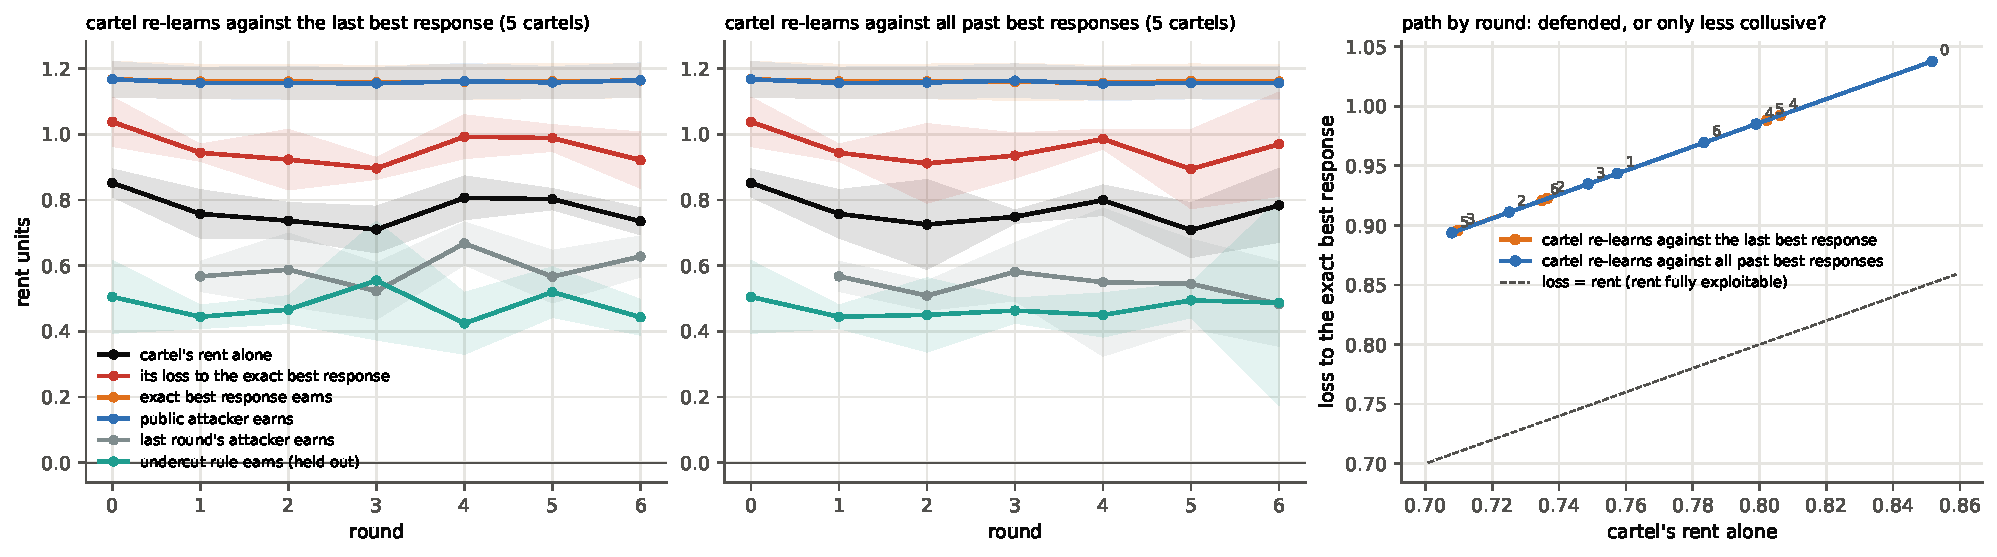
\includegraphics[width=0.98\textwidth]{fig_psro.pdf}
\caption{The double oracle by round and mode; right, the path of (rent, loss to the exact best response) (interim).}\label{fig:psro}
\end{figure}

\textbf{b4. In the queue game there is nothing to steer} (three seeds, preliminary). When the spread is pinned, makers only choose to keep an order standing or step out, and the incumbents are no-regret learners over complete policies. An entrant that behaves one way while they learn and switches afterwards gains nothing: $0.084$ per period against $0.083$ had it been absent. Its presence changes what the incumbents learn (the weight on selecting rises from $0.38$ to $0.68$) but not what it earns ($+0.009$, inside the noise). In the spread game the attacker's take comes from the cartel's reaction; in the queue it comes from selecting takers, and there is no reaction function.

\textbf{b5. A tight request allowance removes the selection rent} (three seeds, preliminary). A maker that selects its fills cancels and re-places orders. With an allowance of placements per 100 periods, plus one per fill: unconstrained, the identity selector earns $+0.10$ per period more than a maker that simply rests and the fringe earns $-0.025$; at an allowance of 2 the edge is $+0.03$; at 1 it is gone ($-0.015$) and the fringe earns $+0.030$. This is the first lever that moves the toxic flow back from identity-blind liquidity to the makers who were avoiding it. Its cost is depth: selectors are locked out in 38--48\% of the periods in which they want to rest. One maker cannot drain another's allowance in this model; the allowance is a tax on selection, not an attack surface.

\textbf{b6. One frontier} (Figure~\ref{fig:frontier}; the strong attackers are being added). Each lever is a point: profit with no attack against profit under the worst attacker. The makers' own levers barely move against the rule attackers, and on the first cartel tested the exact best response and the public attacker leave a defended cartel nothing under every defence. The venue's levers move incumbents along the diagonal. We also now report the customer side: the uninformed taker's expected gain from trade is closed-form in the best quote and is recorded for every defence, alone and under attack.

\begin{figure}[h]\centering
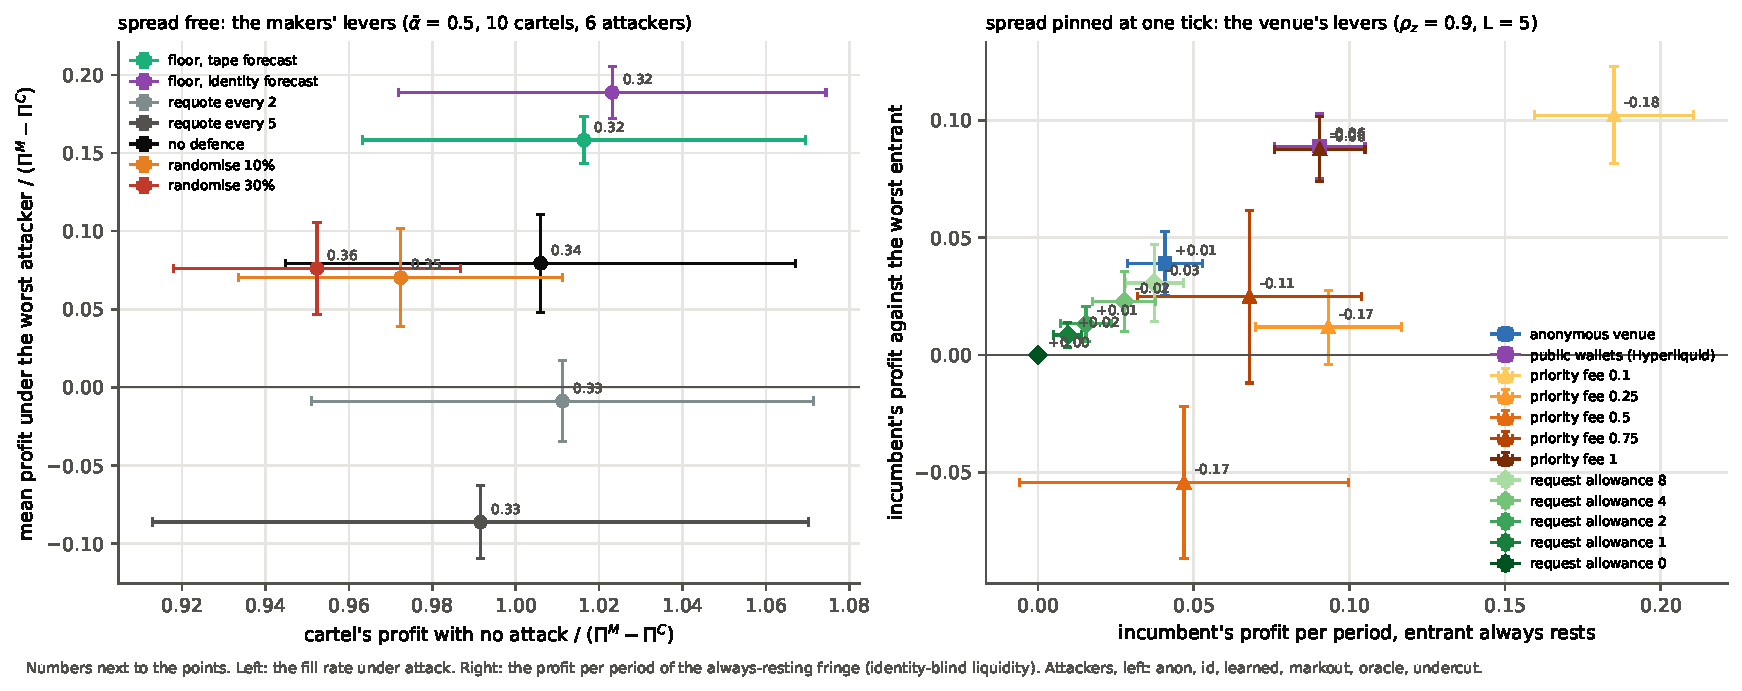
\includegraphics[width=0.98\textwidth]{fig_frontier.pdf}
\caption{Profit alone against profit under the worst attacker. Left: makers' levers, spread mode. Right: venue levers, queue mode.}\label{fig:frontier}
\end{figure}

\textbf{b7. Data} (final for the window Oct 6 -- Nov 1). On fourteen times the Workshop 1 sample the identity-selection gap holds on 33 of 35 coin-days and 94 of 96 coin-hours (the top-10 makers take $1.9$--$3.6\times$ fewer fills from previously toxic wallets), and labels stay valid for at least ten days. In the stress episode of Oct 29 the gap failed on the asset being sold for five hours because one identity-blind wallet absorbed the flow, the queue model's prediction.

\sect{c) Prototype: a visual replay}
\texttt{python experiments/trace.py --all} records nine scenarios from the real simulator and \texttt{demo/index.html} replays them period by period in a browser: the makers' quotes against the Nash and monopoly quotes, each taker's order, the hidden regime, the public tape with delayed marks, and running profit, with play, step, seek, a playback rate from 1 to 200 periods per second, and two runs side by side. The player contains no model logic and a test pins the recording to the experiment code. The repository has 72 tests and one command per figure (\texttt{make figures}).

\sect{d) Limitations}
The results in b2--b6 are from laptop runs on two-maker cartels with few seeds (b2: five per toxicity level); the full grids are scripted (\texttt{slurm/workshop2.sh}). Incumbents are tabular learners; a function-approximation learner may be harder to identify. The queue-game steering result is a null on three seeds. The allowance model charges only placements. Takers are stylised and depth beyond the best price is not modelled.

\sect{e) Plan to the preprint}
(1) Run the five grids at full size and replace the interim numbers. (2) The customer-outcome comparison promised at Workshop 1: taker surplus and fringe profit under each rule, with loss-making participants allowed to leave. (3) December order-level archive: which action carries the selection. (4) Preprint mid-December; the draft is \texttt{paper/arxiv\_draft.tex}.
\end{document}
